The previous Section \ref{}

\begin{table*}[t]
\centering
	\small
\begin{tabular}{ll|rrrr|rrrr|rrrr}
\toprule
&  & \multicolumn{4}{c||}{All objects} & \multicolumn{4}{c||}{MN agreement $>$ 0.9} & \multicolumn{3}{c}{MN agreement $\leq$ 0.9}\\
               model &  GT &  hit &  valid &  err$_{hum}$ &  err &  hit &  valid &   err$_{hum}$ &   err &  hit &  valid &  err$_{hum}$ &  err \\
\midrule
       FRCNN$_{\text{VG1600}}$ &  VG & 74.8 &     13.3 &         7.5 &    4.5 &      94.8 &           0.5 &              2.1 &             2.6 &     63.6 &         20.4 &            10.5 &            5.5 \\
        FRCNN$_{\text{MN442}}$ &  VG & 71.1 &     13.4 &         8.1 &    7.4 &      89.6 &           0.8 &              3.4 &             6.2 &     60.7 &         20.5 &            10.8 &            8.0 \\
 FRCNN$_{\text{VG1600VGMN}}$ &  MN & 80.7 &      8.8 &         7.4 &    3.2 &      94.5 &           0.0 &              4.2 &             1.3 &     72.9 &         13.7 &             9.2 &            4.2 \\
     ResNet101$_{\text{VGMN}}$ &  VG & 62.8 &     11.4 &        15.8 &   10.0 &      88.3 &           0.5 &              5.7 &             5.5 &     48.5 &         17.5 &            21.4 &           12.5 \\
     ResNet101$_{\text{VGMN}}$ &  MN & 68.7 &      9.2 &        13.9 &    8.1 &      89.6 &           0.5 &              4.9 &             4.9 &     57.0 &         14.1 &            19.0 &            9.9 \\
    ResNet101$_{\text{MN442}}$ &  MN & 69.7 &      9.3 &        13.5 &    7.5 &      90.1 &           0.5 &              4.4 &             4.9 &     58.2 &         14.3 &            18.7 &            8.9 \\
    ResNet101$_{\text{MN442}}$ &  VG & 63.8 &     11.6 &        14.8 &    9.8 &      88.6 &           0.8 &              4.4 &             6.2 &     49.9 &         17.6 &            20.7 &           11.8 \\
\bottomrule
\end{tabular}


\caption{New table} \label{tab:humanlike}
\end{table*}


\begin{table*}[t]
\centering
	\small
\begin{tabular}{lrrr||rrr}
\toprule
&  \multicolumn{3}{c||}{MN agreement $>$ 0.9} & \multicolumn{3}{c}{MN agreement $\leq$ 0.9}\\
                  model &  hit &  correct &  incorrect &  hit &  correct &  incorrect \\
\midrule
       FRCNN$_{\text{VG1600}}$\_VG &      94.8 &           1.8 &             3.4 &     63.6 &         24.5 &           12.0 \\
        FRCNN--MN442\_VG &      89.6 &           1.6 &             8.8 &     60.7 &         23.9 &           15.4 \\
        		\midrule \midrule
 FRCNN$_{\text{VG1600}}$$_{\text{VGMN}}$\_MN &      94.5 &           1.3 &             4.2 &     72.9 &         16.5 &           10.6 \\
 		\midrule 
     ResNet101$_{\text{VGMN}}$\_VG &      88.3 &           1.8 &             9.9 &     48.5 &         23.6 &           27.8 \\
     ResNet101$_{\text{VGMN}}$\_MN &      89.6 &           1.6 &             8.8 &     57.0 &         19.4 &           23.6 \\
    ResNet101--MN442\_MN &      90.1 &           1.3 &             8.6 &     58.2 &         19.5 &           22.3 \\
\bottomrule

\end{tabular}
\caption{Break-down of the results (in \%) according to the agreement level of the MN name: Categorization of a predicted name\ $\hat{n}$ into either a \textit{hit}, \textit{correct} (less preferred name, synonym, hypernym/hyponym), or \textit{wrong} \label{tab:exp_errors_agreement}}
\end{table*}

\paragraph{Alternative Name Prediction}
\begin{figure}
	\centering
	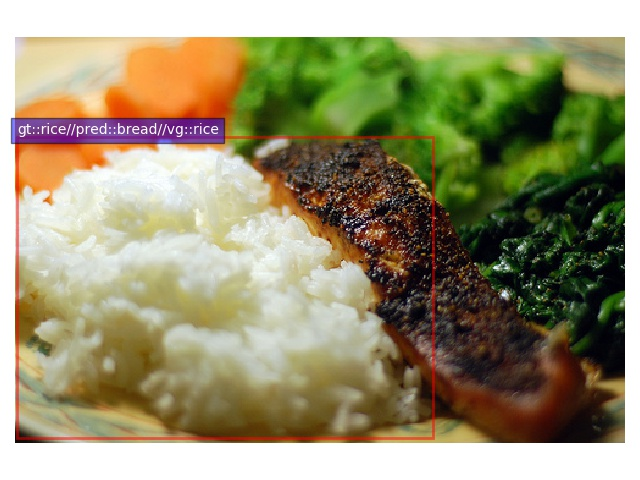
\includegraphics[scale=.2]{images/2323938.jpg}
	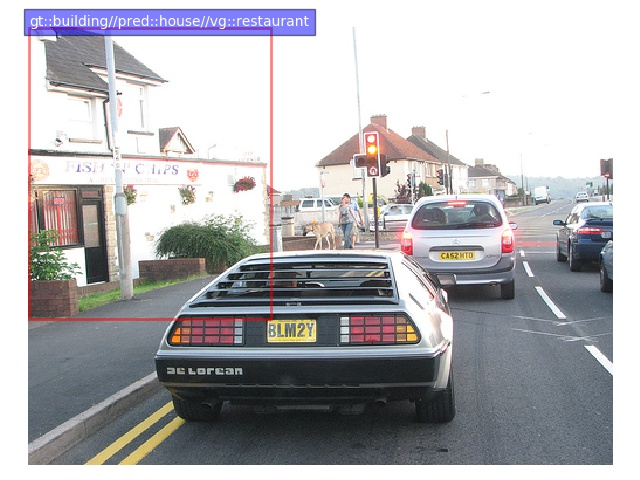
\includegraphics[scale=.2]{images/2322259.jpg}
	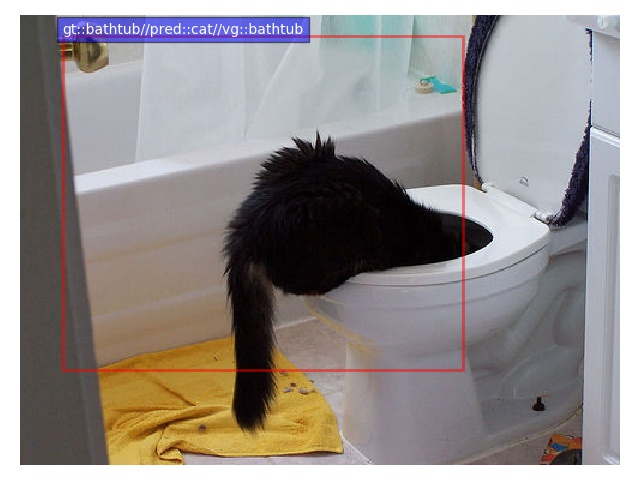
\includegraphics[scale=.2]{images/2371657.jpg}
	
	\caption{TODO: examples resnet mistakes (trained on vg\_manynames, tested on manynames-442)\label{fig:mistakes} \gbt{Will we have space for the figure? (Maybe we should \textit{make} space?) Also, shouldn't we put examples from the most successful model instead?}}
\end{figure}

\cs{TODO::}
Categorization of "errors" (see Figure~\ref{fig:mistakes}):
\begin{enumerate}
	\item Clear mistake \\
	e.g.,\ rice vs. bread
	\item Alternative name\\
	e.g.,\ building vs. house
	\item Alternative object \cs{(other cluster from verif data)}
	\item Synonym\\
	e.g.,\ plane vs. airplane
	\item Semantically related\\
	e.g.,\  motorcycle vs. scooter
\end{enumerate}

\begin{table*}[t]
	\centering
	\small
	\begin{tabular}{l|c|r@{~}|r@{~}r@{~}r@{~}r@{~}r@{~}||r@{~}|r@{~}r@{~}r@{~}r@{~}r@{~}}
		\toprule
		& & \multicolumn{6}{c}{All Test Images ($\#$)} 
		& \multicolumn{6}{c}{VG$\neq$MN Images ($\#$)}\\
		\toprule
		Model$_{\text{Vocab}}$ &  GTtrain & same &  syn. &  syn. &  hyper. &  hypo. &  hyper. &  same &  syn. &  syn. &  hyper. &  hypo. &  hyper. \\
		& 	&  cluster &  & cluster & & & cluster 
		& cluster  &  & cluster & & & cluster \\
		\midrule
		FRCNN$_{\text{VG1600}}$ & VG     %        &                  0.95 &              0.0 &                0.01 &              0.01 &             0.03 &                 0.0 &                  0.96 &              0.0 &                 0.0 &              0.01 &             0.03 &                 0.0 \\
		&                  94.6 &              0.0 &                 0.7 &               3.4 &              1.3 &                  0.0 &                  95.5 &              0.0 &                 0.0 &               3.0 &              1.5 &                  0.0 \\
		FRCNN$_{\text{MN442}}$ & VG %&                   0.97 &             0.01 &                0.02 &               0.0 &              0.0 &                 0.0 &                  0.97 &              0.0 &                0.03 &               0.0 &              0.0 &                 0.0 \\
		&                  93.3 &              1.3 &                 2.0 &               1.3 &              2.0 &                  0.0 &                  93.8 &              0.0 &                 3.1 &               1.6 &              1.6 &                  0.0 \\
		\midrule \midrule
		FRCNN$_{\text{VG1600}}$$_{\text{VGMN}}$ & MN %&                   1.0 &              0.0 &                 0.0 &               0.0 &              0.0 &                 0.0 &                   1.0 &              0.0 &                 0.0 &               0.0 &              0.0 &                 0.0 \\
		&                  94.9 &              0.0 &                 0.0 &               2.0 &              3.0 &                  0.0 &                  96.2 &              0.0 &                 0.0 &               1.9 &              1.9 &                  0.0 \\
		\midrule
		ResNet101$_{\text{VGMN}}$ & MN %&                  0.97 &              0.0 &                0.03 &               0.0 &              0.0 &                 0.0 &                  0.98 &              0.0 &                0.02 &               0.0 &              0.0 &                 0.0 \\
		&                  83.9 &              0.0 &                 2.7 &               6.2 &              5.4 &                  1.8 &                  92.6 &              0.0 &                 1.9 &               1.9 &              3.7 &                  0.0 \\
		ResNet101$_{\text{MN442}}$ & MN %& 0.97 &              0.0 &                0.03 &               0.0 &              0.0 &                 0.0 &                  0.98 &              0.0 &                0.02 &               0.0 &              0.0 &                 0.0 \\
		&                  86.4 &              0.0 &                 2.7 &               5.5 &              3.6 &                  1.8 &                  92.3 &              0.0 &                 1.9 &               1.9 &              3.8 &                  0.0 \\
		ResNet101$_{\text{VGMN}}$ & VG %&                   0.98 &              0.0 &                0.02 &               0.0 &              0.0 &                 0.0 &                  0.98 &              0.0 &                0.02 &               0.0 &              0.0 &                 0.0 \\
		&                  87.4 &              0.0 &                 2.2 &               1.5 &              8.1 &                  0.7 &                  92.5 &              0.0 &                 1.5 &               1.5 &              4.5 &                  0.0 \\
		ResNet101$_{\text{MN442}}$ & VG% &                  0.98 &              0.0 &                0.02 &               0.0 &              0.0 &                 0.0 &                  0.97 &              0.0 &                0.03 &               0.0 &              0.0 &                 0.0 \\		
		&                  88.9 &              0.0 &                 2.2 &               2.2 &              5.9 &                  0.7 &                  92.5 &              0.0 &                 3.0 &               1.5 &              3.0 &                  0.0 \\
		\bottomrule
	\end{tabular}
	
	\caption{Break-down of the results for the \textit{correct} name predictions. Proportions (in \%) of the \textit{correct} categories to all correctly classified instances.  \textit{hyponym}: $\hat{n}$ is a hyponym of the entry-level name. \textit{hypernym\_cl}: $\hat{n}$ is a hypernym of any of the valid names (cluster). \textit{Synonym} and \textit{synonym\_cl} are analogous. \label{tab:exp_alternatives}}
\end{table*}

\paragraph{Incorrect Predictions}

\begin{table*}[t]
	\centering
	\small
	\begin{tabular}{l|c|r@{~}|r@{~}r@{~}r@{~}r@{~}|r@{~}r@{~}||r@{~}|r@{~}r@{~}r@{~}r@{~}|r@{~}r@{~}}
		\toprule
		&& \multicolumn{7}{c}{All Test Images ($\#$)} 
		& \multicolumn{7}{c}{VG$\neq$MN Images ($\#$)}\\
		\toprule
		Model$_{\text{Vocab}}$ & GTtrain  
		&  co- &  \multicolumn{4}{c}{other object}  &  error &  low 
		&  co- &  \multicolumn{4}{c}{other object}  &  error &  low \\
		& & hypo. & (vis. &  ling. &  box &  other)   & & count 
		&  hypo. & (vis. &  ling. &  box &  other) &   & count     \\
		
		\midrule
		FRCNN$_{\text{VG1600}}$ & VG     &                 13.2 &             1.7 &                 0.0 &                  17.4 &            6.6 &           39.7 &             21.5 &                  5.7 &             5.7 &                 0.0 &                  17.1 &           14.3 &           42.9 &             14.3 \\
		FRCNN$_{\text{MN442}}$ & VG       &                 15.5 &             0.6 &                 0.0 &                  15.5 &            6.2 &           49.1 &             13.0 &                  5.9 &             2.0 &                 0.0 &                  13.7 &           11.8 &           54.9 &             11.8 \\
		\midrule \midrule
		FRCNN$_{\text{VG1600}}$$_{\text{VGMN}}$ & MN &                 30.6 &             0.9 &                 0.0 &                  13.0 &            5.6 &           32.4 &             17.6 &                 16.7 &             2.8 &                 0.0 &                  16.7 &           11.1 &           41.7 &             11.1 \\
		\midrule
		ResNet101$_{\text{VGMN}}$ & MN	&                 34.1 &             0.0 &                 0.0 &                  13.0 &            1.3 &           39.5 &             12.1 &                 19.6 &             0.0 &                 0.0 &                  12.5 &            5.4 &           51.8 &             10.7 \\
		ResNet101$_{\text{MN442}}$ & MN  &                 33.0 &             0.0 &                 0.0 &                  14.0 &            1.9 &           37.7 &             13.5 &                 21.1 &             0.0 &                 0.0 &                  15.8 &            7.0 &           43.9 &             12.3 \\
		ResNet101$_{\text{VGMN}}$ & VG  &                 37.6 &             0.0 &                 0.0 &                   6.1 &            2.3 &           41.1 &             12.9 &                 24.4 &             0.0 &                 0.0 &                   3.5 &            5.8 &           45.3 &             20.9 \\
		ResNet101$_{\text{MN442}}$ & VG &                 34.0 &             0.0 &                 0.0 &                   7.5 &            2.8 &           41.9 &             13.8 &                 22.6 &             0.0 &                 0.0 &                   6.0 &            8.3 &           39.3 &             23.8 \\
		\bottomrule
	\end{tabular}
	\caption{Break-down of the results for the \textit{wrong} name predictions. Proportions (in \%) of the corresponding categories to all wrongly classified instances.  \label{tab:exp_details_wrong}}
\end{table*}

\paragraph{Human Object Naming through Transfer-Learning} Figure \ref{fig:exp_confusions} visualizes the change in predictions for  some of our retrained and finetuned models with respect to the object detection baseline (bottom-up-1600). For each object, where the new model predicts a different name than the baseline model, we look at the hit-error categories of the original and new predicted name. Observations:
\begin{itemize}
	\item Retraining faster-rcnn on fewer, entry-level names does not lead to better calibration of entry-level names: more original hits change to same-cluster predictions than the other way round. (top left matrix)
	\item Finetuning the original faster-rcnn on many names recalibrates many decision from same-cluster names to the correct hit. Interestingly, also clear errors are calibrated to perfect hits, whereas hardly any error is changed to same-cluster or related.  (top right matrix)
	\item A similar tendency can be found for the ResNet models: finetuning ResNet on MN changes many predictions from same-cluster to hits. This is less the case when ResNet is finetuned on VG annotations.
	\item Interestingly, both ResNet models change hits into related names (hypernyms, hyponyms, cp-hyponyms) -- why does this happen?
\end{itemize}

\begin{figure*}[t]
	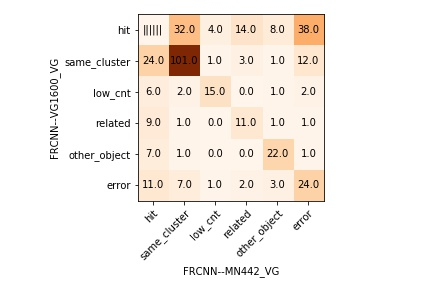
\includegraphics[scale=.5]{images/matrix_FRCNN--VG1600_VG_FRCNN--MN442_VG.jpg}
	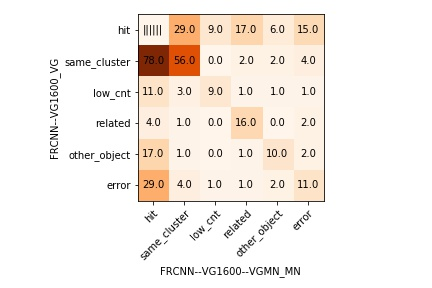
\includegraphics[scale=.5]{images/matrix_FRCNN--VG1600_VG_FRCNN--VG1600--VGMN_MN.jpg}
	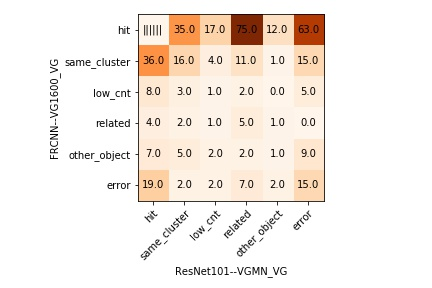
\includegraphics[scale=.5]{images/matrix_FRCNN--VG1600_VG_ResNet101--VGMN_VG.jpg}
	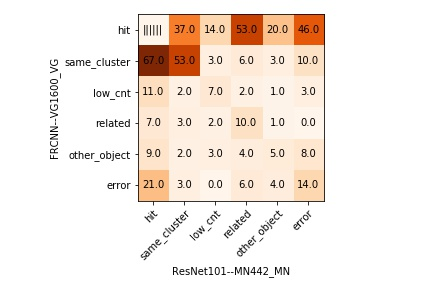
\includegraphics[scale=.5]{images/matrix_FRCNN--VG1600_VG_ResNet101--MN442_MN.jpg}
	
	\caption{Confusion-matrix-style visualization showing error categories of predictions that changed from object detection with FRCNN-VG1600 to naming with FRCNN-VG1600-VGMN (finetuned) \label{fig:exp_confusions}}
\end{figure*}

\subsection{[TBC] Humans vs. Models: Which Mistakes do they Make?}
\label{sect:exp_analysis}

\paragraph{Categorization of Errors}
see Figure\ ref{fig:mistakes}
\begin{enumerate}
	\item Clear mistake \\
	e.g.,\ rice vs. bread
	\item Alternative name\\
	e.g.,\ building vs. house
	\item Alternative object \cs{(other cluster from verif data)}
	\item Synonym\\
	e.g.,\ plane vs. airplane
	\item Semantically related\\
	e.g.,\  motorcycle vs. scooter
\end{enumerate}

\begin{figure}
	\centering
	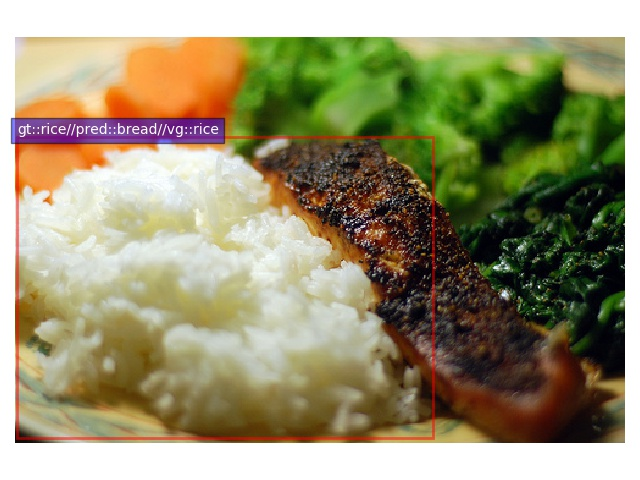
\includegraphics[scale=.2]{images/2323938.jpg}
	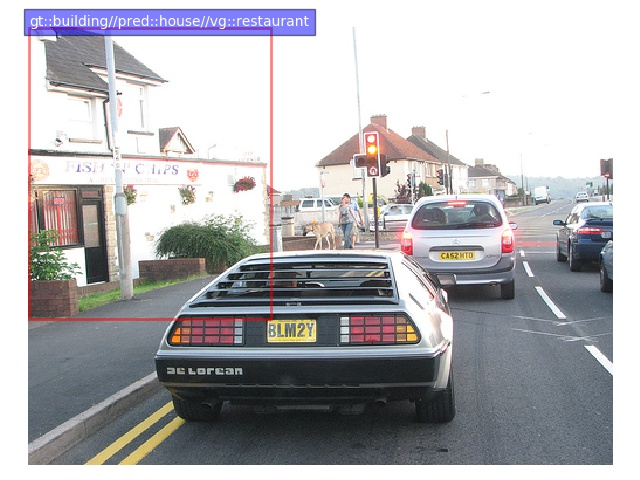
\includegraphics[scale=.2]{images/2322259.jpg}
	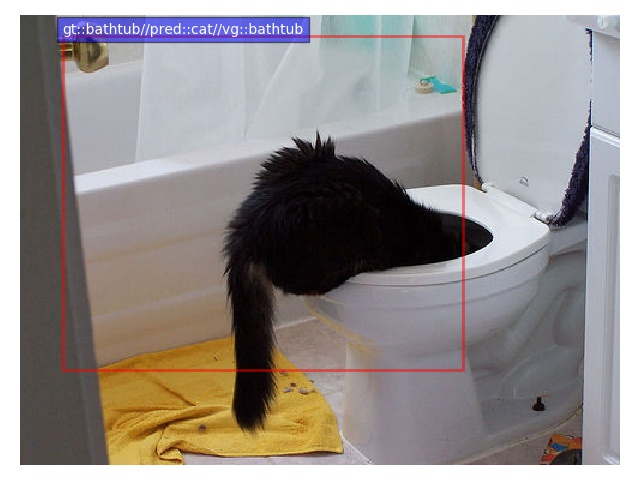
\includegraphics[scale=.2]{images/2371657.jpg}
	
	\caption{resnet mistakes (trained on vg\_manynames, tested on manynames-442)\label{fig:matrices}}
\end{figure}

\subsection{Results}

\paragraph{Overview}
Table\ \ref{tab:exp_overview_results}: \cs{Shows the overview and what MN adds without going into detail: Standard evaluation -- hit; We can additionally distinguish between correct (name alternative, see caption of Table) and clear mistake.}

\paragraph{How do predictions change?} Figure \ref{fig:matrices} visualizes the change in predictions for  some of our retrained and finetuned models with respect to the object detection baseline (bottom-up-1600). For each object, where the new model predicts a different name than the baseline model, we look at the hit-error categories of the original and new predicted name. Observations:
\begin{itemize}
\item Retraining faster-rcnn on less names does not lead to better calibration of entry-level names: more original hits change to same-cluster predictions than the other way round. (top left matrix)
\item Finetuning the original faster-rcnn on many names recalibrates many decision from same-cluster names to the correct hit. Interestingly, also clear errors are calibrated to perfect hits, whereas hardly any error is changed to same-cluster or related.  (top right matrix)
\item A similar tendency can be found for the ResNet models: finetuning ResNet on MN changes many predictions from same-cluster to hits. This is less the case when ResNet is finetuned on VG annotations.
\item Interestingly, both ResNet models change hits into related names (hypernyms, hyponyms, cp-hyponyms) -- why does this happen?
\end{itemize}


\paragraph{Correct predictions}
Table\ \ref{tab:exp_details_correct}: \cs{Gives detailed results to the categories of "correct name" (but not hit): same cluster, WordNet synonym, WordNet hypernym/hyponym}\\
To look into in detail (example images): 
\begin{itemize}
	\item Compare FRCNN vs. FRCNN-finetuned (row block 1 vs. row block 2) with respect to the synonym categories (i.e., predicted name is in a synonym/synonyms\_cluster-relation to the target object) vs. same\_cluster (i.e., predicted name is in response set). 
\end{itemize}

\paragraph{Wrong predictions}

Table\ \ref{tab:exp_details_wrong}: \cs{Gives detailed results to the categories of predicted name\ $\hat{n}$ is incorrect: WordNet co-hyponyms,  other object (inadequacy types: visual, linguistic, bounding box, other (types other+None), $\text{count}(\hat{n})<2$, error (just wrong+unkn(not found in WordNet))}

\begin{table*}[t]
	\centering
	\small
	\begin{tabular}{l|l|r@{~}r@{~}r@{~}||r@{~}r@{~}r@{~}}
		\toprule
		& & \multicolumn{3}{c}{All Test Images ($\#$)} 
		& \multicolumn{3}{c}{VG$\neq$MN Images ($\#$)}\\
	\toprule
	Model$_{\text{Vocab}}$	& GTtrain  
	&  hit &  correct &  incorrect &  hit &  correct &  wrong \\
	\midrule
	FRCNN$_{\text{VG1600}}$ & VG           &         74.8 &                  13.9 &                    11.3 &         54.3 &                  30.0 &                    15.7 \\
	FRCNN--MN442 & VG &         71.1 &                  13.9 &                    15.0 &         48.4 &                  28.7 &                    22.9 \\
	\midrule \midrule
	FRCNN$_{\text{VG1600}}$$_{\text{VGMN}}$ & MN %&         0.81 &                  0.09 &                    0.11 &         0.60 &                  0.23 &                    0.17 \\
	 &         80.7 &                   9.2 &                    10.1 &         60.1 &                  23.8 &                    16.1 \\
	\midrule
	ResNet101--MN442 & MN %& 0.70 &                  0.09 &                    0.21 &         0.51 &                  0.22 &                    0.27 \\
	 &         69.7 &                  10.3 &                    20.1 &         51.1 &                  23.3 &                    25.6 \\
	ResNet101$_{\text{VGMN}}$ & MN% &         0.69 &                  0.09 &                    0.22 &         0.51 &                  0.23 &                    0.26 \\	
	 &         68.7 &                  10.5 &                    20.8 &         50.7 &                  24.2 &                    25.1 \\
	ResNet101$_{\text{VGMN}}$ & VG %&         0.63 &                  0.11 &                    0.26 &         0.31 &                  0.28 &                    0.40 \\
	 &         62.8 &                  12.6 &                    24.6 &         31.4 &                  30.0 &                    38.6 \\
	ResNet101--MN442 & VG %&         0.64 &                  0.11 &                    0.25 &         0.32 &                  0.29 &                    0.39 \\
	 &         63.8 &                  12.6 &                    23.6 &         32.3 &                  30.0 &                    37.7 \\
	\bottomrule
\end{tabular}
\caption{Break-down of the results (in \%): Categorization of a predicted name\ $\hat{n}$ into either a \textit{hit} (exact match with entry-level name, cf. standard evaluation), \textit{correct} (less preferred name, synonym, hypernym/hyponym), or \textit{wrong} (wrong object, $\text{count}(\hat{n})<2$, co-hyponym, clear mistake). \label{tab:exp_overview_results}}
\end{table*}

%%% Local Variables:
%%% mode: latex
%%% TeX-master: "acl2020_main"
%%% End:
